\documentclass[tikz]{standalone}
\usepackage{wasysym}
\usepackage{SIunits}
\usepackage{pgfplots}
\pgfplotsset{compat=1.5}
\usetikzlibrary{plotmarks,arrows}
\tikzset{>=latex}
\definecolor{tissueColour}{RGB}{251,185,130}
\definecolor{lesionColour}{RGB}{175,50,53}
\begin{document}
	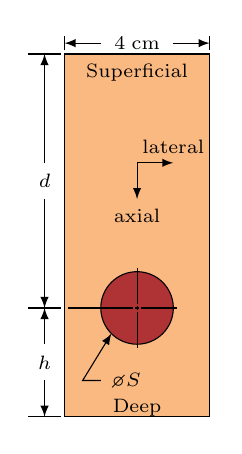
\begin{tikzpicture}[x=0.038\textwidth, y=0.038\textwidth, draw=black, text=black, fill=black]
		% the main domain area
		\draw[fill=tissueColour] (0, 0) rectangle(4, 10);

		% the lesion
		\draw[fill=lesionColour] (2, 3) circle(1);

		% the lesion size
		%\draw[<-] (2.707, 3.707) -- (3, 4) -- (3.9, 4);
		%\draw (4.1, 4) -- (4.5, 4) node[right]{$\diameter S$};
		\draw[<-] (1.293, 2.293) -- (0.5, 1) -- (1, 1) node[right]{\scriptsize $\diameter S$};

		% the lesion locator
		\draw (0.1, 3) -- (1.9, 3);
		\draw (2.1, 3) -- (3.1, 3);
		\draw (2, 1.9) -- (2, 2.9);
		\draw (2, 3.1) -- (2, 4.1);
		\draw (2, 2.95) -- (2, 3.05);
		\draw (1.95, 3) -- (2.05, 3);

		% lesion depth
		\draw (-1, 10) -- (-0.1, 10);
		\draw (-1, 3) -- (-0.1, 3);
		\draw (-0.55, 6.5) node{\scriptsize $d$};
		\draw[<-] (-0.551, 10) -- (-0.551, 7);
		\draw[->] (-0.551, 6) -- (-0.551, 3);

		% lesion bottom separation
		\draw (-1, 0) -- (-0.1, 0);
		\draw (-0.55, 1.5) node{\scriptsize $h$};
		\draw[<-] (-0.55, 3) -- (-0.55, 2);
		\draw[->] (-0.55, 1) -- (-0.55, 0);

		% domain width
		\draw (0, 10.1) -- (0, 10.5);
		\draw (4, 10.1) -- (4, 10.5);
		\draw (2, 10.3) node{\scriptsize $\unit{4}{cm}$};
		\draw[<-] (0, 10.3) -- (1, 10.3);
		\draw[->] (3, 10.3) -- (4, 10.3);

		% directions
		\draw[<->] (2, 6) node[below]{\scriptsize axial} -- (2, 7) -- (3, 7) node[above]{\scriptsize lateral};
		\draw (2, 9.5) node{\scriptsize Superficial};
		\draw (2, 0.25) node{\scriptsize Deep};
	\end{tikzpicture}
\end{document}